\documentclass[12pt]{article}
\usepackage[utf8]{inputenc}
\usepackage{amsmath}
\usepackage{graphicx}
\usepackage[left=2cm, right=2.50cm, top=2.50cm, bottom=2.50cm]{geometry}
\author{Carolina Valenzuela Córdova}
\title{\LaTeX}
\date{}
\begin{document}
\title{Reporte Producto 7: Descripción de actividades}
\maketitle{}






La marea es el cambio periódico del nivel del mar producido principalmente por la fuerza de atracción gravitatoria que ejercen el Sol y la Luna sobre la Tierra. Aunque dicha atracción se ejerce sobre todo el planeta, tanto en su parte sólida como líquida y gaseosa, nos referiremos en este artículo a la atracción de la Luna y el Sol, juntos o por separado, sobre las aguas de los mares y océanos. Sin embargo, hay que indicar que las mareas de la litosfera son prácticamente insignificantes, con respecto a las que ocurren en el mar u océano (que pueden modificar su nivel en varios metros) y, sobre todo, en la atmósfera, donde puede variar en varios km de altura, aunque en este caso, es mucho mayor el aumento del espesor de la atmósfera producido por la fuerza centrífuga del movimiento de rotación en la zona ecuatorial (donde el espesor de la atmósfera es mucho mayor) que la modificación introducida por las mareas en dicha zona ecuatorial.\\

 El fenómeno de las mareas es conocido desde la antigüedad. Parece ser que Piteas fue el primero en señalar la relación entre la amplitud de la marea y las fases de la Luna, así como su periodicidad. Plinio el Viejo en su Naturalis Historia describe correctamente el fenómeno y piensa que la marea está relacionada con la Luna y el Sol. Mucho más tarde, Bacon, Kepler y otros trataron de explicar ese fenómeno, admitiendo la atracción de la Luna y del Sol. Pero fue Isaac Newton en su obra Philosophiae Naturalis Principia Mathematica uien dio la explicación de las mareas aceptada actualmente. Más tarde, Pierre Simon-A continuación se recogen los principales términos empleados en la descripción de las mareas:

Marea alta o pleamar: momento en que el agua del mar alcanza su máxima altura dentro del ciclo de las mareas.
Marea baja o bajamar: momento opuesto, en que el mar alcanza su menor altura.Laplace y otros científicos ampliaron el estudio de las mareas desde un punto de vista dinámico.
 Isaac Newton realizó varios estudios científicos del comportamiento de las mareas y calculó la altura de éstas según la fecha del mes, la estación del año y la latitud. Más tarde, Simon Laplace complementó los estudios de Newton.\\


A continuación se recogen los principales términos empleados en la descripción de las mareas:

*Marea alta o pleamar: momento en que el agua del mar alcanza su máxima altura dentro del ciclo de las mareas.\\
*Marea baja o bajamar: momento opuesto, en que el mar alcanza su menor altura.
El tiempo aproximado entre una pleamar y la bajamar es de 6 horas, completando un ciclo de 24 horas 50 minutos.\\
En la última actividad del curso, se analizó un un conjunto de series de tiempo de un sensor que mide: Fecha (mm/dd/aaaa), tiempo (cada 30min), presión (kPa), temperatura del agua (ºC), nivel del mar (metros) y día del año (DOY=Day of Year: 1-365). Tenemos un archivo con datos, que nos ha proporcionado el Dr. Julio César Rodríguez, del Departamento de Agricultura. Los datos se proporcionan en un archivo en formato de Excel, el cual fue necesario modificar para que el programa producido en Fortran puediera leerlo y graficarlo.
Algunas modificaciones consistieron en cambiar el formato de las horas, adecuar el conteo de los días y acomodar todos los datos en columnas pertinentes para que el programa graficara solamente lo que necesitamos, es decir, todas las mareas mínimas y máximas.
Además, como parte de la actividad, también se pedía calcular distancias entre valles y crestas de las gráficas obtenidas a lo largo de la misma.\\

A continuación se presenta una gráfica obtenida con el programa producido de todos los datos proporcionados por el archivo en excel:

 
 *Código final:\\
 \begin{verbatim}
 
 Program Mareas
Implicit None

real, dimension (1:7674) :: Altura
real :: Max1, Max2, Max3, Max4, Max5,Min1, Min2, Min3, Min4, Min5
real :: Tiempo1M, Tiempo2M, Tiempo3M, Tiempo4M, Tiempo5M, Tiempo1MIN, Tiempo2MIN
real :: Tiempo3MIN, Tiempo4MIN, Tiempo5MIN, Periodomax1, Periodomax2, Periodomax3, k
real :: Periodomax4, Periodomin1, Periodomin2, Periodomin3, Periodomin4, Promax, Promin
real:: Maxdiurno1, Maxdiurno2, Maxdiurno3, Maxdiurno4
real :: Maxnocturno1, Maxnocturno2, Maxnocturno3, Maxnocturno4
real :: TiempoMaxdiurno1,TiempoMaxdiurno2,TiempoMaxdiurno3,TiempoMaxdiurno4
real :: TiempoMaxnocturno1,TiempoMaxnocturno2,TiempoMaxnocturno3,TiempoMaxnocturno4
real:: Periodomaxdiurno1,Periodomaxdiurno2,
Periodomaxdiurno3,Periodomaxnocturno1, Periodomaxnocturno2, Periodomaxnocturno3
real :: Promaxdiurno, Promaxnocturno
integer :: i

open (1, file="Mareas.csv")
do i=1, 7674
read (1,*) Altura (i)
end do
close (1)

Max1=0
do i=1, 1440
k= Max1-Altura(i)
if (k<0) then
Max1= Altura(i)
Tiempo1M=i/48.00
end if
end do
 
Max2=0
do i=1441, 2880
k=Max2-Altura(i)
if (k<0) then
Max2= Altura(i)
Tiempo2M=i/48.00

end if
end do

Max3=0
do i=2881,4320
k= Max3-Altura(i)
if (k<0) then
Max3= Altura (i)
Tiempo3M=i/48.00
end if
end do

Max4=0
do i=4321,5761
k= Max4-Altura(i)
if (k<0) then
Max4= Altura (i)
Tiempo4M=i/48.00
end if
end do

Max5=0
do i=5762,7202
k= Max5-Altura(i)
if (k<0) then
Max5= Altura(i)
Tiempo5M=i/48.00
end if
end do










Min1=0
do i=1, 1440
k= Min1-Altura(i)
if (k>0) then
Min1= Altura(i)
Tiempo1MIN=i/48.00
end if
end do

Min2=0
do i=1441, 2880
k=Min2-Altura(i)
if (k>0) then
Min2= Altura(i)
Tiempo2MIN=i/48.00

end if
end do

Min3=0
do i=2881,4320
k= Min3-Altura(i)
if (k>0) then
Min3= Altura (i)
Tiempo3MIN=i/48.00
end if
end do

Min4=0
do i=4321,5761
k= Min4-Altura(i)
if (k>0) then
Min4= Altura (i)
Tiempo4MIN=i/48.00
end if
end do

Min5=0
do i=5762,7202
k= Min5-Altura(i)
if (k>0) then
Min5= Altura(i)
Tiempo5MIN=i/48.00
end if
end do


Maxdiurno1=0
do i=1,24
k=Maxdiurno1-Altura(i)
if (k<0) then
Maxdiurno1= Altura (i)
TiempoMaxdiurno1= i*0.5
end if
end do 

Maxnocturno1=0
do i=25,48
k=Maxnocturno1-Altura(i)
if (k<0) then
Maxnocturno1= Altura(i)
TiempoMaxnocturno1= i*0.5
end if
end do

Maxdiurno2=0
do i=49,73
k=Maxdiurno2-Altura(i)
if (k<0) then
Maxdiurno2= Altura (i)
TiempoMaxdiurno2= i*0.5
end if
end do 


Maxnocturno2=0
do i=74,98
k= Maxnocturno2-Altura(i)
if (k<0) then
Maxnocturno2= Altura(i)
TiempoMaxnocturno2= i*0.5
end if 
end do


Maxdiurno3=0
do i=99,123
k= Maxdiurno3-Altura(i)
if (k<0) then
Maxdiurno3= Altura(i)
TiempoMaxdiurno3= i*0.5
end if
end do 

Maxnocturno3=0
do i=124,148
k= Maxnocturno3-Altura(i)
if (k<0) then
Maxnocturno3= Altura(i)
TiempoMaxnocturno3= i*0.5
end if 
end do

Maxdiurno4=0
do i=149,173
k= Maxdiurno4-Altura(i)
if (k<0) then
Maxdiurno4= Altura(i)
TiempoMaxdiurno4= i*0.5
end if
end do 


Maxnocturno4=0
do i=174,198
k= Maxnocturno4-Altura(i)
if (k<0) then
Maxnocturno4= Altura(i)
TiempoMaxnocturno4= i*0.5
end if 
end do






Periodomax1= (Tiempo2M-Tiempo1M)
Periodomax2= (Tiempo3M-Tiempo2M)
Periodomax3= (Tiempo4M-Tiempo3M)
Periodomax4= (Tiempo5M-Tiempo4M)
Periodomin1= (Tiempo2MIN-Tiempo1MIN)
Periodomin2= (Tiempo3MIN-Tiempo2MIN)
Periodomin3= (Tiempo4MIN-Tiempo3MIN)
Periodomin4= (Tiempo5MIN-Tiempo4MIN)
Promax= ((Periodomax1+Periodomax2+Periodomax3+Periodomax4)/4)
Promin= ((Periodomin1+Periodomin2+Periodomin3+Periodomin4)/4)
Periodomaxdiurno1= (TiempoMaxdiurno2-TiempoMaxdiurno1)
Periodomaxdiurno2= (TiempoMaxdiurno3-TiempoMaxdiurno2)
Periodomaxdiurno3= (TiempoMaxdiurno4-TiempoMaxdiurno3)
Periodomaxnocturno1= (TiempoMaxnocturno2-TiempoMaxnocturno1)
Periodomaxnocturno2= (TiempoMaxnocturno3-TiempoMaxnocturno2)
Periodomaxnocturno3= (TiempoMaxnocturno4-TiempoMaxnocturno3)
promaxdiurno = ((Periodomaxdiurno1+Periodomaxdiurno2+Periodomaxdiurno3)/3)
promaxnocturno = ((Periodomaxnocturno1+Periodomaxnocturno2+Periodomaxnocturno3)/3)

Print *, 'Las mareas maximas de los cinco meses son', Max1, Max2, Max3, Max4, Max5
Print *, 'Las mareas minimas de los cinco meses son', Min1, Min2, Min3, Min4, Min5
Print *,'Tiempos de las mareas maximas', Tiempo1M, 
Tiempo2M, Tiempo3M, Tiempo4M, Tiempo5M
Print *, 'Tiempo de las mareas minimas', Tiempo1MIN,
 Tiempo2MIN, Tiempo3MIN, Tiempo4MIN, Tiempo5MIN
Print *, 'Periodos de maximos', Periodomax1, Periodomax2, Periodomax3, Periodomax4
Print *, 'Periodos de minimos', Periodomin1, Periodomin2, Periodomin3, Periodomin4
Print *, 'Promedio de periodos de las mareas maximas', Promax
Print *, 'Promedio de periodos de las mareas minimos', Promin
Print *, 'Las mareas maximas diurnas de cinco dias son',
 Maxdiurno1,Maxdiurno2,
Maxdiurno3,Maxdiurno4
Print *, 'Las mareas maximas nocturnas de cinco dias son', 
Maxnocturno1, Maxnocturno2, Maxnocturno3, Maxnocturno4
Print *, 'Tiempos de mareas maximas diurnas', TiempoMaxdiurno1,TiempoMaxdiurno2,
TiempoMaxdiurno3,TiempoMaxdiurno4
Print *, 'Tiempos de mareas maximas nocturnas', TiempoMaxnocturno1,TiempoMaxnocturno2,
TiempoMaxnocturno3,TiempoMaxnocturno4
Print *, 'Periodos de maximos diurnos',Periodomaxdiurno1,
Periodomaxdiurno2,Periodomaxdiurno3
Print *, 'Periodos de maximos nocturnos',
Periodomaxnocturno1, Periodomaxnocturno2, Periodomaxnocturno3
Print *, 'Promedio de periodos de maximos diurnos',Promaxdiurno
Print *, 'Promedio de periodos de maximos nocturnos', Promaxnocturno

end Program Mareas
\end{verbatim}

Resultados numéricos obtenidos por el programa:
\begin{verbatim}
Las mareas maximas de los cinco meses son   1.15499997      0.885999978      
 1.09899998       1.08599997       1.09099996    
 Las mareas minimas de los cinco meses son -0.275999993     -0.625999987    
  -0.564999998     -0.418500006     -0.389999986    
 Tiempos de las mareas maximas   21.4791660       51.5000000       80.5000000     
   109.500000       138.479172    
 Tiempo de las mareas minimas   13.0000000       45.0833321       74.1666641       
 105.229164       148.083328    
 Periodos de maximos   30.0208340       29.0000000       29.0000000      
  28.9791718    
 Periodos de minimos   32.0833321       29.0833321       31.0625000      
  42.8541641    
 Promedio de periodos de las mareas maximas   29.2500019    
 Promedio de periodos de las mareas minimos   33.7708321    
 Las mareas maximas diurnas de cinco dias son   4.89999987E-02  0.326000005     
  0.588000000      0.764999986    
 Las mareas maximas nocturnas de cinco dias son  0.579999983      0.697000027     
  0.717000008      0.644999981    
 Tiempos de mareas maximas diurnas   7.50000000       32.5000000      
  57.5000000       82.0000000    
 Tiempos de mareas maximas nocturnas   20.5000000       45.0000000     
   69.5000000       94.0000000    
 Periodos de maximos diurnos   25.0000000       25.0000000       24.5000000    
 Periodos de maximos nocturnos   24.5000000       24.5000000       24.5000000    
 Promedio de periodos de maximos diurnos   24.8333340    
 Promedio de periodos de maximos nocturnos   24.5000000    
\end{verbatim}



 \begin{figure}[H]
 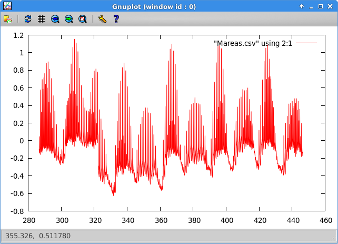
\includegraphics{General}
 \centering
 \caption{Gráfica de todas las mareas registradas por el archivo }
 \end{figure}
 
 En conclusión, las mareas altas y bajas varían día con día pues como la posición relativa de la luna y del sol varían con el tiempo, el tamaño y la ubicación de la marea también cambia. Esto se debe a que la marea se propaga como una onda, puesto que la tierra gira sobre sí misma, es el efecto de rotación el que hace que cada día en las costas de todo el planeta exista mareas bajas y altas dos veces al día. 



\end{document}